\usetikzlibrary{positioning}

\begin{document}

\def\title{Worksheet 8}

\newcommand{\qitem}{\qpart\item}

\renewcommand{\labelenumi}{(\alph{enumi})} % change default enum format to (a)
\renewcommand{\theenumi}{(\alph{enumi})} % fix reference format accordingly.
\renewcommand{\labelenumii}{\roman{enumii}.} % second level labels.
\renewcommand{\theenumii}{\roman{enumii}.}

\maketitle

\vspace{0.5em}

\begin{qunlist}
\qns{Transfer Function}

Create a Bode plot of the following transfer function:

$$H(\omega) = \frac{1}{10} \frac{((j\omega)^2 + 110j\omega + 1000)(j\omega + 10000)}
	{(j\omega+1000)((j\omega)^2 + 101j\omega + 100)}$$

\sol{

First of all, we decompose the second-order terms:
$$H(\omega) = \frac{1}{10} \frac{((j\omega)+100)(j\omega+10))(j\omega + 10000)}
	{(j\omega+1000)((j\omega)+100)(j\omega+1))}  =
		 \frac{1}{10} \frac{(j\omega+10)(j\omega + 10000)}
	{(j\omega+1000)(j\omega+1)}$$
Then, we convert it to the normal form:
$$H(\omega) =
		 \frac{10}{1} \frac{(\frac{j\omega}{10}+1)(\frac{j\omega}{10000} + 1)}
	{(\frac{j\omega}{1000}+1)(j\omega+1)}$$
	
\begin{figure}[H]
\centering
\scalebox{0.9}{\includegraphics[scale=0.6]{\bank/transfer/figures/q_complicated_fixed.png}}
\end{figure}

}

\newpage
% Author: Alexander Feng

\qns{RLC Bandstop Filter}

One way to compose a bandpass filter is by combining a low pass and high pass filter via a buffer.
Another way to compose a bandpass is to use a RLC circuit of the following form:

\begin{figure}[h!]
\begin{center}
\begin{circuitikz}[american]
    \node[ground](g){};
    \draw (g) to[sV, l = $V_{in}(t)$] ++ (0, 3) coordinate(input);
    \draw (input) -- ++(1, 0) to[C, l = $C$] ++ (0.5, 0) coordinate(capacitor);
    \draw (capacitor) -- ++(0.5, 0) to[L, l = $L$] ++(2, 0) coordinate(output) -- ++(1, 0) node[ocirc]{$ . V_{out}(t)$};
    \draw (output) to[R, l = $R$] ++(0, -3) node[ground]{};
\end{circuitikz}
\end{center}
\caption{RLC Bandpass Filter}
\end{figure}

Let's explore what happens when swap the location of the resistor with the location of the capacitor and inductor.

\begin{figure}[h!]
% Author: Alexander Feng Fall 2020
\begin{center}
\begin{circuitikz}[american voltages]
    \draw node[ground]{} (0,0) to[sV, l = $V_{in}(t)$, invert]
    (0,3) -- (0.25, 3) to[R = $R$] (3, 3) -- (4, 3) node[ocirc]{$ . V_{out}(t)$};
    \draw (3,3) to[C, C = $C$] (3, 1.5) to[L, L = $L$] (3,0) node[ground]{};
\end{circuitikz}
\end{center}

\caption{Unknown Behavior}
\end{figure}

\begin{enumerate}

\qitem
Write out the transfer function of figure 2.

\meta{
See if you can get students to guess what the behavior will ultimately be based on the topology of the circuit and what their knowledge of resonancy tells them so far.
In particular, during resonancy, the impedance of circuit elements cancel each other and cause a short.
In the bandpass, this results in $Vout(t)$ being directly connected to the voltage source.
In the bandstop, it results in a short to ground!
}

\sol{
Note that $j = -\frac{1}{j}$.
This can be proved by multiplying both sides by $j$.
Thus,
\begin{align*}
H_{notch}(j\omega) = \frac{j(L\omega - \frac{1}{C\omega})}{R + j(L\omega - \frac{1}{C\omega})}
\end{align*}
}

\qitem
What is the magnitude of the transfer function?

\sol{
\begin{align*}
\left | H_{notch}(j\omega) \right | =
\frac{\sqrt{(L\omega - \frac{1}{C\omega})^{2}}}{\sqrt{R^{2} + (L\omega - \frac{1}{Cw})^{2}}}
\end{align*}
}

\qitem
Sketch the magnitude of this transfer function.

\sol{
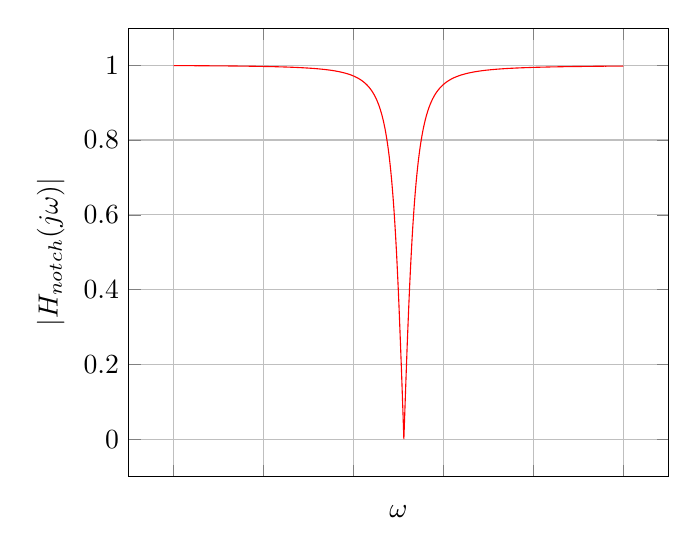
\begin{tikzpicture}
\begin{axis}[
xlabel={$\omega$},
ylabel={$|H_{notch}(j\omega)|$},
grid=major,
xticklabels = {}]
\addplot[domain=250:500, color = red, samples = 550]  {(((0.07 * x - ((1)/(0.0001 * x)))^2)^0.5)/((1 + ((0.07 * x) - (1)/(0.0001 * x))^2)^0.5)};
\end{axis}
\end{tikzpicture}

Notice that the magnitude of the transfer function is approximately one outside of some very small region.
}

\qitem
When is the magnitude of the transfer function zero?
When is it one?

\sol{
The magnitude of the transfer function is zero precisely when
\begin{align*}
L\omega = \frac{1}{C\omega}
\end{align*}
}

\qitem
How would you describe the behavior of this circuit?
Why do you think circuits with this type of circuit behavior are classified as notch/bandstop filters?
Why is this specific filter called a \emph{resonsant} bandstop filter?


\sol{
The circuit's behavior can be thought of as the complement or opposite to the bandpass filter.
While the bandpass filter allows a range of frequencies through, the bandstop/notch stops a particular range of frequencies from passing through.
This is also why it'd be called bandstop or notch.
Bandstop is opposite of bandpass.
Notch comes from how the graph of the magnitude looks like there's a notch.
This filter is a specific type of bandstop filter in that it's resonant.
Resonance occurs when at a specific frequencies, the impedances of circuit elements cancel each other.
For this circuit, this occurs when $L\omega = \frac{1}{C\omega}$.
}




\end{enumerate}

\newpage

\qns{Bode Plots for Filters}
\pgfplotsset{compat=1.9, every tick label/.append style={font=\normalsize}} 

\meta{Prereqs: Transfer Functions, Complex magnitude and phases, plotting functions}

Bode plots provide us with a simple and easy tool to plot these transfer functions by hand. \textbf{Always remember that Bode plots are an approximation}; if you want the precisely correct plots, you need to use numerical methods (like solving using MATLAB or IPython).

When we make Bode plots, we plot the frequency and magintude on a logarithmic scale and the angle in either degrees or radians. 
We use the log scale because it allows us to break up complex transfer functions into its constituent components. 

% We note that every transfer function can be written in its \textit{rational transfer function form,} which is a product of poles and zeros. When making the Bode plot (and plotting using a logarithmic unit), we treat each individual pole and zero independently, and then add them back together at the end. This question will examine the Bode plots of single zeros and poles, and we can generalize these plots to create a Bode plot for any transfer function.

When plotting the transfer function, the most important quantity to look at is its cutoff frequency $\omega_{c}.$ 
We will take a look the individual Bode plots for low and high pass filters, and then look at how the Bode plot for a bandpass filter is constructed. 

\meta{
  Note: This semester, drawing straight-line approximations to Bode plots are no longer in scope.
  However, we will motivate the process of drawing straight line approximations by looking at points for which $\omega \approx 0, \omega = \omega_c,$ and $\omega >> \omega_c.$
}

\begin{enumerate}
\qitem Consider a circuit with transfer function: 
  $H(\omega) = \frac{1}{j\omega C_{1}R_{1} + 1} \cdot \frac{j\omega C_{2}R_{2}}{j\omega C_{2}R_{2} + 1}$
\begin{enumerate}
  \qitem What are the cutoff frequencies of this filter?
  \ws{\vspace{60px}}
  \sol{
  The lower cutoff is the cutoff frequency of the high-pass filter:
  $$\omega_{c,l} = \frac{1}{R_{2}C_{2}} = 10^{5}$$
  The upper cutoff is the cutoff frequency of the low-pass filter:
  $$\omega_{c,u} = \frac{1}{R_{1}C_{1}} = 10^{8}$$
  }
  \qitem Sketch its phase and magnitude. \textit{Hint: How can we combine the plots of the individual filters together?}

  \sol{
  For both the magnitude and the phase plots, you can "add" the plots of the high-pass filter and the low-pass filter.
  This can be done since both are on a log-log scale.
  
  \begin{figure}[h]
  \textbf{Magnitude plot:}
  \centering
    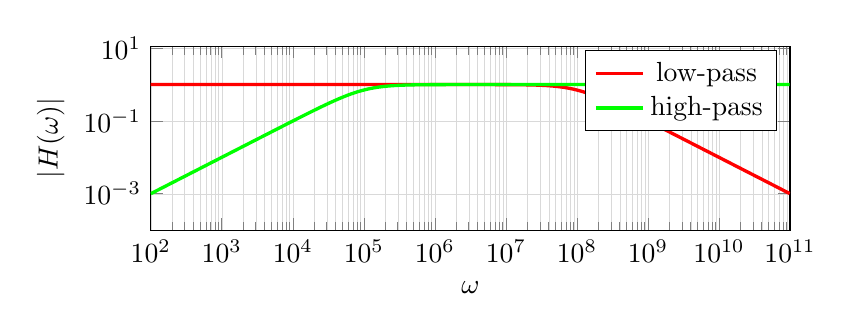
\begin{tikzpicture}[
      declare function={
         highpass(\omega)= (\omega / 10^5) * sqrt(1 + (\omega / 10^5)^2) / (1 + (\omega / 10^5)^2)
        % highpass(\omega)= (\omega < 10^5) * (\omega / 10^5) +
        %           (\omega >= 10^5) * (1)
        ;
        lowpass(\omega)= 1 / sqrt(1 + (\omega / 10^8)^2)
         % lowpass(\omega)= (\omega < 10^8) * (1) +
         %           (\omega >= 10^8) * (10^8 / \omega)
        ;
        }
    ]
      \begin{loglogaxis}[
        ymin=0.0001, ymax=11, ylabel=$|H(\omega)|$,
        xmin=10^2, xmax=10^11, xlabel=$\omega$,
        domain=10^2:10^11,
        grid=both, grid style={line width=.1pt, draw=gray!30},
        width=\textwidth * 0.8,
        height=\textwidth / 3.1,
        samples=800
      ]
        \addplot [red,very thick] {lowpass(x)};
        \addlegendentry{low-pass}
        \addplot [green,very thick] {highpass(x)};
        \addlegendentry{high-pass}
      \end{loglogaxis}
    \end{tikzpicture}
  \end{figure}

  \begin{figure}
  \centering
    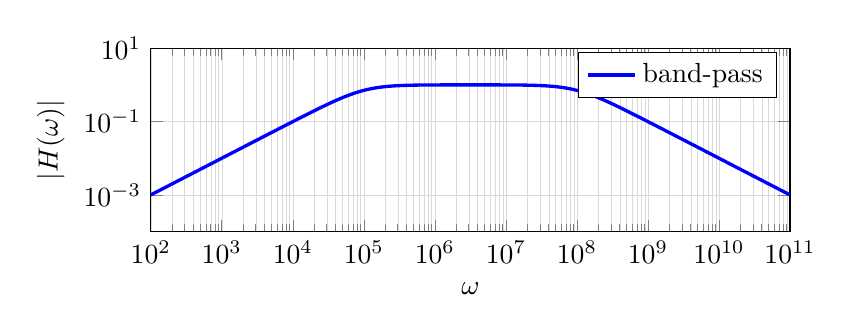
\begin{tikzpicture}[
      declare function={
      highpass(\omega)= (\omega / 10^5) / sqrt(1 + (\omega / 10^5)^2)
      % highpass(\omega)= (\omega < 10^5) * (\omega / 10^5) +
      %           (\omega >= 10^5) * (1)
      ;
      lowpass(\omega)= 1 / sqrt(1 + (\omega / 10^8)^2)
       % lowpass(\omega)= (\omega < 10^8) * (1) +
       %           (\omega >= 10^8) * (10^8 / \omega)
      ;
      }
    ]
      \begin{loglogaxis}[
        ymin=0.0001, ymax=10, ylabel=$|H(\omega)|$,
        xmin=10^2, xmax=10^11, xlabel=$\omega$,
        domain=10^2:10^11,
        grid=both, grid style={line width=.1pt, draw=gray!30},
        width=\textwidth * 0.8,
        height=\textwidth / 3.1,
        samples=300
      ]
        \addplot [blue,very thick] {lowpass(x) * highpass(x)};
        \addlegendentry{band-pass}
        
      \end{loglogaxis}
    \end{tikzpicture}
  \end{figure}

  \begin{figure}[!h]
  \textbf{Phase plot:}
  \centering

    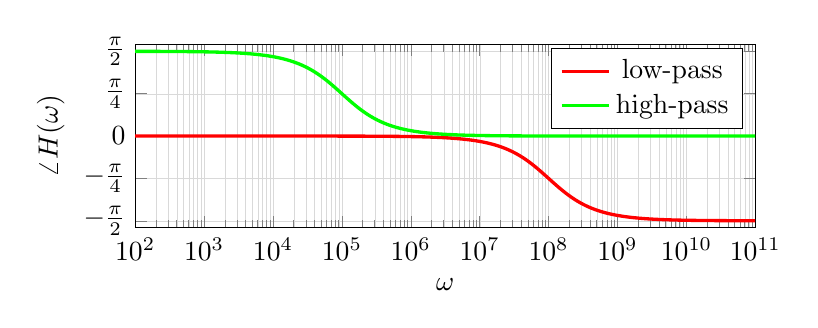
\begin{tikzpicture}[
      declare function={
      lowpass(\omega) = -rad(atan(\omega / 10^8))
        % lowpass(\omega)= (\omega < 10^7) * (0) +
        %           and(\omega >= 10^7, \omega < 10^9) * (-pi / 4 * (log10(\omega) - 7)) +
        %           (\omega >= 10^9) * (-pi / 2)
       ;
      highpass(\omega) = pi/2 - rad(atan(\omega / 10^5))
       % highpass(\omega)= (\omega < 10^4) * (pi / 2) +
       %           and(\omega >= 10^4, \omega < 10^6) * (-pi / 4 * (log10(\omega) - 4) + pi / 2) +
       %           (\omega >= 10^6) * (0)
      ;
      }
    ]

      \begin{semilogxaxis}[
        ymin= -1.7, ymax=1.7, ylabel=$\angle H(\omega)$,
        ytick={-pi/2, -pi/4, 0, pi/4, pi/2},
        yticklabels={$-\frac{\pi}{2}$,$-\frac{\pi}{4}$,$0$,$\frac{\pi}{4}$,$\frac{\pi}{2}$},
        xmin=10^2, xmax=10^11, xlabel=$\omega$,
        domain=10^2:10^11,
        grid=both, grid style={line width=.1pt, draw=gray!30},
        width=\textwidth * 0.78,
        height=\textwidth / 3.1,
        samples=500
      ]
        \addplot [red,very thick] {lowpass(x)};
        \addlegendentry{low-pass}
        \addplot [green,very thick] {highpass(x)};
        \addlegendentry{high-pass}
      \end{semilogxaxis}
  \end{tikzpicture}
\end{figure}

\begin{figure}[!h]
\centering

  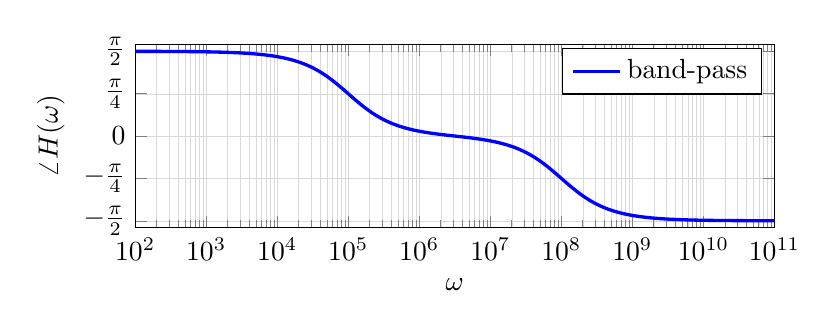
\begin{tikzpicture}[
    declare function={
    lowpass(\omega) = -rad(atan(\omega / 10^8))
      % lowpass(\omega)= (\omega < 10^7) * (0) +
      %           and(\omega >= 10^7, \omega < 10^9) * (-pi / 4 * (log10(\omega) - 7)) +
      %           (\omega >= 10^9) * (-pi / 2)
     ;
    highpass(\omega) = pi/2 - rad(atan(\omega / 10^5))
     % highpass(\omega)= (\omega < 10^4) * (pi / 2) +
     %           and(\omega >= 10^4, \omega < 10^6) * (-pi / 4 * (log10(\omega) - 4) + pi / 2) +
     %           (\omega >= 10^6) * (0)
    ;
    }
  ]

    \begin{semilogxaxis}[
      ymin= -1.7, ymax=1.7, ylabel=$\angle H(\omega)$,
      ytick={-pi/2, -pi/4, 0, pi/4, pi/2},
      yticklabels={$-\frac{\pi}{2}$,$-\frac{\pi}{4}$,$0$,$\frac{\pi}{4}$,$\frac{\pi}{2}$},
      xmin=10^2, xmax=10^11, xlabel=$\omega$,
      domain=10^2:10^11,
      grid=both, grid style={line width=.1pt, draw=gray!30},
      width=\textwidth * 0.8,
      height=\textwidth / 3.1,
      samples=900
    ]
    \addplot [blue,very thick] {lowpass(x) + highpass(x)};
    \addlegendentry{band-pass}
    \end{semilogxaxis}
  \end{tikzpicture}
  \end{figure}
  }
  \meta{
  We can "add" the magnitudes of the high-pass and low-pass filters together because we are graphing $log(|H(\omega)|) = log(|H_{high}(\omega)| \cdot |H_{low}(\omega)|) = log(|H_{high}(\omega)|) + log(|H_{low}(\omega)|)$. \vskip 1pt
  We can "add" the phases because $\angle(H_{high}(\omega) * H_{low}(\omega)) = \angle(H_{high}(\omega)) + \angle(H_{low}(\omega))$.
  }
  \end{enumerate}
\end{enumerate}
Now lets take a look at two more concepts, \textbf{bandwidth} and \textbf{Q-factor}. The bandwidth of a resonance
circuit is the difference between its upper and lower cutoff frequencies. It can also be expressed as \textit{resonance frequency} divided by its \textit{Q-factor}:

\begin{align}
    bandwidth = \Delta \omega = f_{high} - f_{low} = \frac{\omega_n}{Q}
\end{align}

The Q-factor, or quality factor, of a circuit is the ratio of power stored to power dissipated, but can also be more simply thought of as the measure of how good a circuit is,
where a higher Q-factor is often more desirable. This can be expressed mathematically as:

\begin{align}
    Q = \frac{\omega_{n}}{\Delta \omega}
\end{align}

\meta{
Circuits that have low bandwidths relative to their center frequency will have higher Q-factors.
}

\begin{enumerate}[resume]
  \qitem Find the bandwidth of this circuit.
  \ws{\vspace{60px}}
  \sol{
  $$\Delta \omega = \omega_{c,u} - \omega_{c,l} = \frac{1}{R_{1}C_{1}} - \frac{1}{R_{2}C_{2}}$$
  $$\Delta \omega = 10^{8} - 10^{5} = 9.99 \cdot 10^{7}$$
  }
  \qitem What is its Q-factor? I.e.: $\frac{\omega_{n}}{\Delta \omega}$, where $\omega_{n}$ is the center frequency of the band.
  \ws{\vspace{60px}}
  \sol{
  Symbolically:
  $$Q = \frac{\omega_{n}}{\Delta \omega} = \frac{\frac{1}{2}  \cdot (\frac{1}{R_{1}C_{1}} + \frac{1}{R_{2}C_{2}})}{\frac{1}{R_{1}C_{1}} - \frac{1}{R_{2}C_{2}}}$$
  $$Q = \frac{(R_{2}C_{2} + R_{1}C_{1})}{2 \cdot (R_{2}C_{2} - R_{1}C_{1})}$$
  Numerically:
  $$Q = \frac{\omega_{n}}{\Delta \omega} = \frac{1/2 (10^{8} + 10^{5})}{9.99 \cdot 10^{7}} = \frac{5.005 \cdot 10^{7}}{9.99 \cdot 10^{7}}$$
  $$Q \approx 0.501$$
  }
\end{enumerate}
% \end{enumerate}

\newpage
% Authors: Taejin Hwang, Justin Yu
% Emails: taejin@berkeley.edu, justinvyu@berkeley.edu

% Note: This specific reboot is specific to Sahai's Fall 2019 iteration of 16B. It was created by merging the bode_plots_intro and bode_filters question. For future semesters, it'll probably be more appropriate to use the two together.

\qns{Frequency Responses}
\pgfplotsset{compat=1.9, every tick label/.append style={font=\normalsize}} 

The transfer function of a circuit is defined as

\begin{equation}
H(j \omega) = \frac{\widetilde{V}_{out}}{\widetilde{V}_{in}}
\end{equation}

The transfer function depends on the frequency of the input voltage, and will be a complex number for a given frequency. 

When looking at filters, we will define a transfer function that explains the input-output relation for any given frequency and analyze its behavior. 
For the purposes of this question, we will consider various filter configurations, and study their behavior.

\begin{enumerate}

\qitem Given the following filter, with $R = 100 \Omega$ and $C = 100 pF,$

\begin{center}
  \begin{circuitikz} \draw
    (0, 0) node[ground] {}
      to [sV, l_=$V_{in}$] (0, 4)
      to [R = R] (4, 4)
      to [C = C] (4, 0)
      node[ground] {}

    (4, 3) to[short, -o] (6, 3) node[anchor=west] (A) {A}

    (4, 1) to[short, -o] (6, 1) node[anchor=west] (B) {B}

    (A) to[open, l^=$V_{out}$] (B)
  ;\end{circuitikz}
\end{center}


\begin{enumerate}[label=(\roman*)]
  \item \textbf{Write out the transfer function $H(j\omega)$.}
  \item \textbf{For values of $\omega$ approaching $0$, find $\abs{H(j\omega)}$.}
  \item \textbf{For values of $\omega$ approaching $\infty$, find $\abs{H(j\omega)}$.}
  \item \textbf{What is the cutoff frequency of this filter?}
  \item \textbf{Sketch its phase and magnitude.}
\end{enumerate}

\sol {

\begin{enumerate}[label=(\roman*)]
  \item The circuit can be simplified as:
    \input{\bank/filters/filter_transfer/fig_simplified_low_pass}

    We recognize the circuit is a voltage divider.
    Let $\widetilde{V}_{out}$ and $\widetilde{V}_{in}$ be voltage phasors.
    Using the voltage divider equation with impedance, we have
    \[
      \widetilde{V}_{out} = \frac{Z_C}{Z_R + Z_C}\widetilde{V}_{in} = H(j\omega)\widetilde{V}_{in}
    .\]
    Notice that the above equation uses impedance and voltage phasors instead of resistance and voltage.
    From the above equation, the circuit has the transfer function
    \[
      H(j\omega) = \frac{Z_C}{Z_R + Z_C}
      = \frac{\frac{1}{j\omega C}}{R + \frac{1}{j\omega C}}
      = \frac{1}{1 + j\omega RC}
    ,\]

  \item For values of $\omega$ close to $0$, $\abs{H(j\omega)}$ approaches $1$.
    In this case, $\widetilde{V}_{out} = \widetilde{V}_{in}$, meaning that low frequencies will pass through this filter.

  \item For values of $\omega$ approaching $\infty$, $\abs{H(j\omega)}$ approaches $0$.
    In this case, $\widetilde{V}_{out} = 0$, meaning that high frequencies will be attenuated by this filter.
    
    \vspace{0.1 cm} 

    Since this filter allows low frequencies to go through and blocks high frequencies, it is called a \emph{low-pass filter}.

  \item Recall that the cutoff frequency is the point at which the magnitude of $H(j \omega)$ is equal to $\frac{1}{\sqrt{2}}.$ 
  The reason for this values is since it is the "half-power" point. Since $H(j \omega) = \frac{1}{1 + j \omega RC},$ and noting that $\frac{1}{1 + j}$ has magnitude $\frac{1}{\sqrt{2}},$ we can solve for $\omega$ and get $\omega_{c} = \frac{1}{RC} = \frac{1}{10^{2} \cdot 10^{-10}} = 10^{8}$

  \item {
  Magnitude (log-log scale): The magnitude of $H(j \omega)$ is close to 1 until $\omega_{c}$, after which it starts decreasing at a quick rate.

  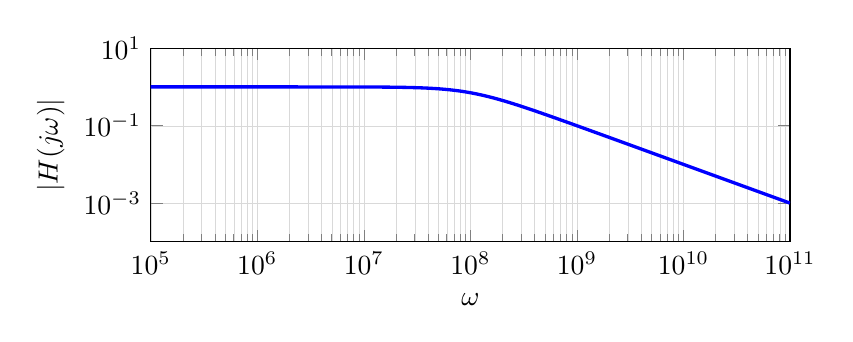
\begin{tikzpicture}[
    declare function={
      mag(\omega)= 1 / sqrt(1 + (\omega / 10^8)^2)
      % Bode approximation
      % (\omega < 10^8) * (1) +
      %           (\omega >= 10^8) * (10^8 / \omega)
     ;
    }
  ]
    \begin{loglogaxis}[
      ymin=0.0001, ymax=10, ylabel=$|H(j \omega)|$,
      xmin=10^5, xmax=10^11, xlabel=$\omega$,
      domain=10^5:10^11,
      grid=both, grid style={line width=.1pt, draw=gray!30},
      width=\textwidth * 0.8,
      height=\textwidth / 3,
      samples=800
    ]
      \addplot [blue,very thick] {mag(x)};
    \end{loglogaxis}
  \end{tikzpicture}
  
  Phase (semi-log scale): The phase of $H(j \omega)$ can be approximated using the three points from the previous parts. When $\omega << \omega_{c}, \angle H(j \omega) = 0,$ when $\omega = \omega_{c}, \angle H(j \omega) = \frac{\pi}{4},$ and when $\omega >> \omega_{c}, \angle H(j \omega) = \frac{\pi}{2}.$

  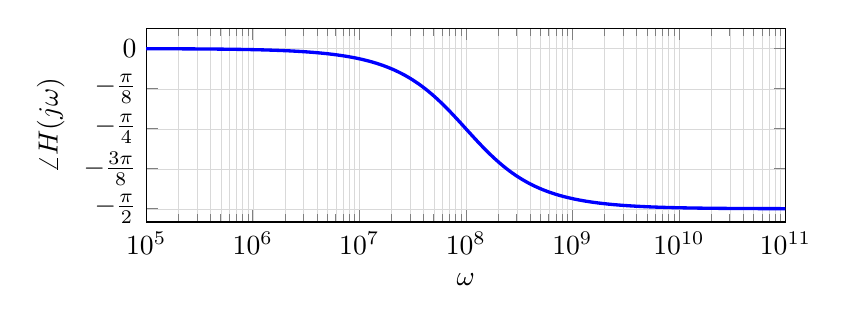
\begin{tikzpicture}[
    declare function={
      phase(\omega)= -rad(atan(\omega / 10^8))
      % Bode approximation
      % phase(\omega)= (\omega < 10^7) * (0) +
      %           and(\omega >= 10^7, \omega < 10^9) * (-pi / 4 * (log10(\omega) - 7)) +
      %           (\omega >= 10^9) * (-pi / 2)
      ;
    }
  ]
    \begin{semilogxaxis}[
      ymin= -1.7, ymax=0.2, ylabel=$\angle H(j \omega)$,
      ytick={-pi/2, -3*pi/8, -pi/4, -pi/8, 0},
      yticklabels={$-\frac{\pi}{2}$,$-\frac{3\pi}{8}$,$-\frac{\pi}{4}$,$-\frac{\pi}{8}$,$0$},
      xmin=10^5, xmax=10^11, xlabel=$\omega$,
      domain=10^5:10^11,
      grid=both, grid style={line width=.1pt, draw=gray!30},
      width=\textwidth * 0.8,
      height=\textwidth / 3,
      samples=800
    ]
      \addplot [blue,very thick] {phase(x)};
    \end{semilogxaxis}
  \end{tikzpicture}
  }
\end{enumerate}
}

\qitem Given the following filter, with $R = \SI{1}{\kilo\ohm}$ and $C = \SI{10}{\nano\farad},$

\begin{center}
  \begin{circuitikz} \draw
    (0, 0) node[ground] {}
      to [sV, l_=$v_{in}$] (0, 2)
      to [C = C] (4, 2)
      to [R = R] (4, 0)
      node[ground] {}

    (4, 2) to[short, -o] (5, 2) node[anchor=west] (A) {A}

    (4, 0) to[short, -o] (5, 0) node[anchor=west] (B) {B}

    (A) to[open, l^=$v_{out}$] (B)
  ;\end{circuitikz}
\end{center}


\begin{enumerate}[label=(\roman*)]
  \item \textbf{Write out the transfer function $H(j\omega)$.}
  \item \textbf{For values of $\omega$ approaching $0$, find $\abs{H(j\omega)}$.}
  \item \textbf{For values of $\omega$ approaching $\infty$, find $\abs{H(j\omega)}$.}
  \item \textbf{What is the cutoff frequency of this filter?}
  \item \textbf{Sketch its phase and magnitude.}
\end{enumerate}

\sol {
\begin{enumerate}[label=(\roman*)]
   \item The circuit can be simplified as:

    \begin{center}
  \begin{circuitikz}[american] \draw
    (0, 0) to[C, l=$C$] (2, 0) to[R, l=$R$] (2, -2) node[ground] {}
    (2, 0) to (3, 0) node[ocirc] {} node[right] {$V_{out}$}
    (0, 0) node[ocirc] {} node[left] {$V_{in}$}
  ;\end{circuitikz}
\end{center}


    Using the voltage divider equation with impedance, we have
    \[
      \widetilde{V}_{out} = \frac{Z_R}{Z_R + Z_C}\widetilde{V}_{in} = H(j \omega)\widetilde{V}_{in}
    .\]

    Thus, the circuit has the transfer function

    \[
      H(j \omega) = \frac{Z_R}{Z_R + Z_C}
      = \frac{R}{R + \frac{1}{j\omega C}}
      = \frac{j\omega RC}{1 + j\omega RC}
    .\]

  \item For values of $\omega$ close to $0$, $\abs{H(j \omega)}$ approaches $0$.
    In this case, $\widetilde{V}_{out} = 0$, it means that low frequencies will be attenuated by this filter.

  \item For values of $\omega$ approaching $\infty$, $\abs{H(j \omega)}$ approaches $1$.
    In this case, $\widetilde{V}_{out} = \widetilde{V}_{in}$, meaning high frequencies will pass through this filter.

    \vspace{0.1 cm} 

    Since this filter allows high frequencies to go through and blocks low frequencies, it is called a \emph{high-pass filter}.

  \item Doing a similar analysis as before, we can calculate $\omega_{c} = \frac{1}{RC} = \frac{1}{10^{3} \cdot 10^{-8}} = 10^{5}$

  \item 
  Magnitude (log-log scale): The magnitude of $H(j \omega)$ is close to 0 for $\omega$ close to 0. It will increase at a very slow rate

  until $\omega_{c}$, after which it starts increasing at a quick rate, but will asymptotically reach $1$ as $\omega >> \omega_{c}.$

  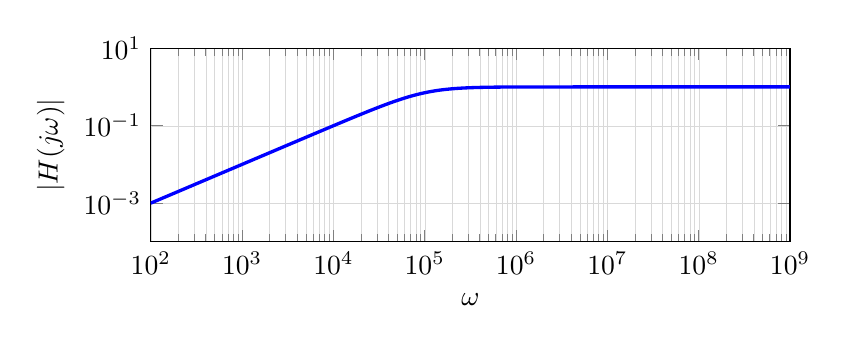
\begin{tikzpicture}[
    declare function={
    mag(\omega)= (\omega / 10^5) / sqrt(1 + (\omega / 10^5)^2)    
     %  Bode approximation
     %  mag(\omega)= (\omega < 10^5) * (\omega / 10^5) +
     %            (\omega >= 10^5) * (1)
     %
     ;
    }
  ]
    \begin{loglogaxis}[
      ymin=0.0001, ymax=10, ylabel=$|H(j \omega)|$,
      xmin=10^2, xmax=10^9, xlabel=$\omega$,
      domain=10^2:10^9,
      grid=both, grid style={line width=.1pt, draw=gray!30},
      width=\textwidth * 0.8,
      height=\textwidth / 3,
      samples=500
    ]
      \addplot [blue,very thick] {mag(x)};
    \end{loglogaxis}
    \vspace{0.3 cm}
  \end{tikzpicture}
  
  Phase (semi-log scale): The phase of $H(j \omega)$ is $\frac{\pi}{2}$ for $\omega << \omega_{c}.$ When $\omega = \omega_{c}, \angle H(j \omega) = \frac{\pi}{4},$ for larger values of $\omega,$ it will continue to decreases until it asymptotically reaches $0$ as $\omega >> \omega_{c}.$

  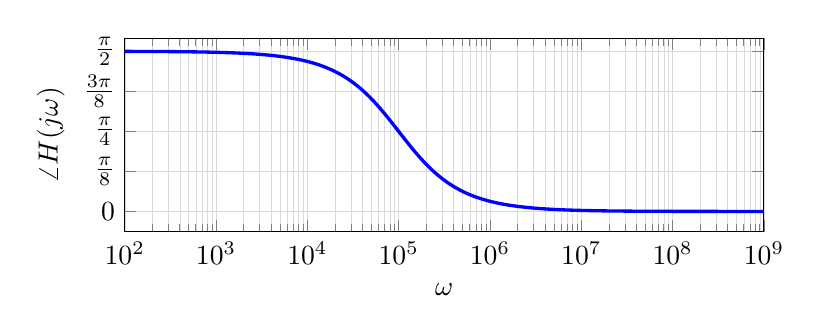
\begin{tikzpicture}[
    declare function={
    phase(\omega)= pi/2 - rad(atan(\omega / 10^5))
      % Bode approximation 
      % phase(\omega)= (\omega < 10^4) * (pi / 2) +
      %           and(\omega >= 10^4, \omega < 10^6) * (-pi / 4 * (log10(\omega) - 4) + pi / 2) +
      %           (\omega >= 10^6) * (0)
     ;
    }
  ]
  \begin{semilogxaxis}[
    ymin= -0.2, ymax=1.7, ylabel=$\angle H(j \omega)$,
    ytick={pi/2, 3*pi/8, pi/4, pi/8, 0},
    yticklabels={$\frac{\pi}{2}$,$\frac{3\pi}{8}$,$\frac{\pi}{4}$,$\frac{\pi}{8}$,$0$},
    xmin=10^2, xmax=10^9, xlabel=$\omega$,
    domain=10^2:10^9,
    grid=both, grid style={line width=.1pt, draw=gray!30},
    width=\textwidth * 0.8,
    height=\textwidth / 3,
    samples=500
  ]
    \addplot [blue,very thick] {phase(x)};
  \end{semilogxaxis}
\end{tikzpicture}

\end{enumerate}
}

\qitem Given the following filter, with $R_{1} = \SI{100}{\ohm}, R_{2} = \SI{1}{\kilo\ohm}$ and $C_{1} = \SI{100}{\pico\farad}, C_{2} = \SI{10}{\nano\farad},$

\begin{center}
  \begin{circuitikz} \draw
    (0, 2) node[ground] (lground) {}
      to [sV, l_=$v_{in}$] (0, 4)
      to [R = $R_1$] (4, 4)
      to [C = $C_1$] (4, 2)
      node[ground] (mground) {}

    (7, 3.5) node[op amp, yscale=-1] (opamp) {}
      (opamp.+) to [short] (4, 4)
      (opamp.-) -| (5.5, 2)
      (opamp.out) |- (5.5, 2)
      (opamp.out) to [C = $C_2$] (12, 3.5)
      to [R = $R_2$] (12, 0.5)
      node[ground] (rground) {}

    (12, 3.5) to[short, -o] (14, 3.5) node[anchor=west] (A) {A}

    (12, 1) to[short, -o] (14, 1) node[anchor=west] (B) {B}

    (A) to[open, l^=$v_{out}$] (B)
  ;\end{circuitikz}
\end{center}


\begin{enumerate}[label=(\roman*)]
  \item \textbf{Write out the transfer function $H(j\omega)$.}
  \item \textbf{For values of $\omega$ approaching $0$, find $\abs{H(j\omega)}$.}
  \item \textbf{For values of $\omega$ approaching $\infty$, find $\abs{H(j\omega)}$.}
  \item \textbf{What is the cutoff frequency of this filter?}
  \item \textbf{Sketch its phase and magnitude.}
\end{enumerate}

\sol {

\begin{enumerate}[label=(\roman*)]
\item The circuit can be simplified as:

    \begin{center}
  \begin{circuitikz}[american] \draw
    (5, -0.5) node[op amp, yscale=-1](opamp){}
    (0, 0) to[R, l=$R_1$] (2, 0) to[C, l=$C_1$] (2, -2) node[ground] {}
    (2, 0) to (3, 0) node[ocirc] {} node[above] {$V_{center}$} to (opamp.+)
    (0, 0) node[ocirc] {} node[left] {$V_{in}$}
    (6.5, 0) to[C, C=$C_2$] (8.5, 0) to[R, l=$R_2$] (8.5, -2) node[ground] {}
    (8.5, 0) to (9.5, 0) node[ocirc] {} node[right] {$V_{out}$}
    (0, 0) node[ocirc] {} node[left] {$V_{in}$}
    (opamp.-) to (3.5, -1) to (3.5, -2) to (6.5, -2) to (6.5, -0.5) to (opamp.out)
    (6.5, -0.5) to (6.5, 0)
  ;\end{circuitikz}
\end{center}


    In this circuit, the op-amp acts as a unity gain buffer which connects the two filters together.
    On the left of the op-amp is a low-pass filter, and on the right of the op-amp is a high-pass filter.
    Let $H_1(j \omega)$ and $H_2(j \omega)$ be transfer functions for the low-pass and high-pass filters respectively.
    We can write $\widetilde{V}_{out}$ in terms of $H_1(j \omega)$, $H_2(j \omega)$, and $\widetilde{V}_{in}$
    \[
      \widetilde{V}_{out} = H_1(j \omega)H_2(j \omega)\widetilde{V}_{in}
    .\]

    Thus, the circuit has the transfer function

    \[
      H(j \omega) = H_1(j \omega)H_2(j \omega) = \frac{1}{1 + j \omega R_{1}C_{1}} \frac{j \omega R_{2}C_{2}}{1 + j \omega R_{2}C_{2}}
    .\]


  \item Using the above transfer function, we have
    \[
      \abs{H(j \omega)} = \abs{H_1(j \omega)H_2(j \omega)}
      = \abs{H_1(j \omega)}\abs{H_2(j \omega)}
    .\]
    Since $H_1(j \omega)$ is a transfer function of a low-pass filter and $H_2(j \omega)$ is a transfer function of a high-pass filter, for values of $\omega$ approaching $0$, $\abs{H(j \omega)}$ approaches $0$.
    Therefore, $\widetilde{V}_{out} = 0$, meaning low frequencies are attenuated by this filter.

  \item For values of $\omega$ approaching $\infty$, $\abs{H(j \omega)}$ also approaches $0$.
    Therefore, $\widetilde{V}_{out} = 0$; meaning high frequencies are also attenuated by this filter. 

    \vspace{0.1 cm} 
    
    Since this filter blocks both low and high frequencies, and it allows signals of a certain frequency range (a band of frequencies) to pass through, it is called a \emph{band-pass filter}.
  \item What are the cutoff frequencies of this filter?

    The lower cutoff is the cutoff frequency of the high-pass filter:
    $$\omega_{c,h} = \frac{1}{R_{2}C_{2}} = 10^{5}$$
    The upper cutoff is the cutoff frequency of the low-pass filter:
    $$\omega_{c,l} = \frac{1}{R_{1}C_{1}} = 10^{8}$$
  \item Sketch its phase and magnitude. \textit{Hint: How can we combine the plots of the individual filters together?}

    For both the magnitude and the phase plots, you can "add" the plots of the high-pass filter and the low-pass filter.
    This can be done since both are on a log-log scale.
    \begin{figure}[h]
    \textbf{Magnitude plot:}
    \centering
      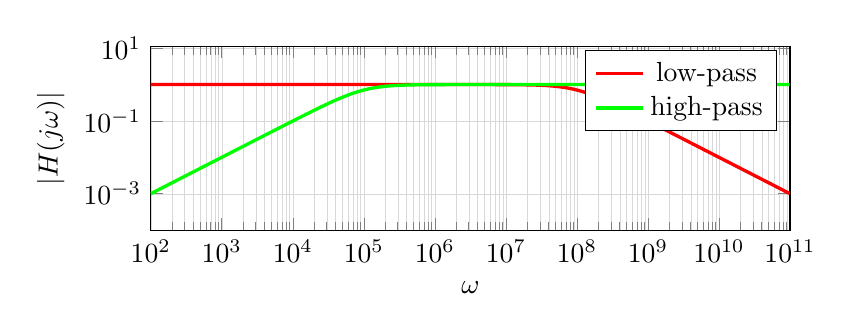
\begin{tikzpicture}[
        declare function={
         highpass(\omega)= (\omega / 10^5) * sqrt(1 + (\omega / 10^5)^2) / (1 + (\omega / 10^5)^2)
        % highpass(\omega)= (\omega < 10^5) * (\omega / 10^5) +
        %           (\omega >= 10^5) * (1)
        ;
        lowpass(\omega)= 1 / sqrt(1 + (\omega / 10^8)^2)
         % lowpass(\omega)= (\omega < 10^8) * (1) +
         %           (\omega >= 10^8) * (10^8 / \omega)
        ;
        }
      ]
        \begin{loglogaxis}[
          ymin=0.0001, ymax=11, ylabel=$|H(j \omega)|$,
          xmin=10^2, xmax=10^11, xlabel=$\omega$,
          domain=10^2:10^11,
          grid=both, grid style={line width=.1pt, draw=gray!30},
          width=\textwidth * 0.8,
          height=\textwidth / 3.1,
          samples=800
        ]
          \addplot [red,very thick] {lowpass(x)};
          \addlegendentry{low-pass}
          \addplot [green,very thick] {highpass(x)};
          \addlegendentry{high-pass}
        \end{loglogaxis}
      \end{tikzpicture}
    \end{figure}

    \begin{figure}
    \centering
      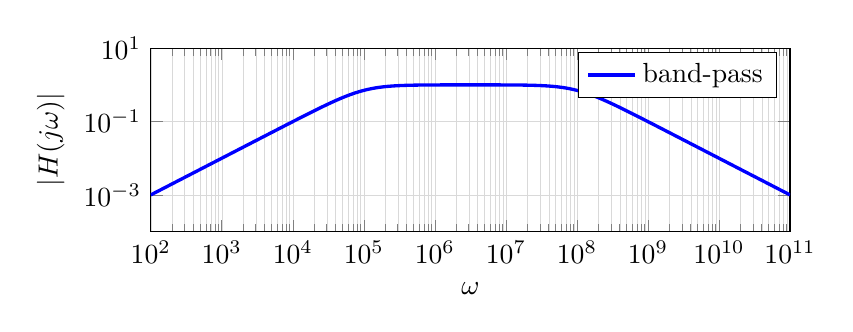
\begin{tikzpicture}[
        declare function={
        highpass(\omega)= (\omega / 10^5) / sqrt(1 + (\omega / 10^5)^2)
        % highpass(\omega)= (\omega < 10^5) * (\omega / 10^5) +
        %           (\omega >= 10^5) * (1)
        ;
        lowpass(\omega)= 1 / sqrt(1 + (\omega / 10^8)^2)
         % lowpass(\omega)= (\omega < 10^8) * (1) +
         %           (\omega >= 10^8) * (10^8 / \omega)
        ;
        }
      ]
        \begin{loglogaxis}[
          ymin=0.0001, ymax=10, ylabel=$|H(j \omega)|$,
          xmin=10^2, xmax=10^11, xlabel=$\omega$,
          domain=10^2:10^11,
          grid=both, grid style={line width=.1pt, draw=gray!30},
          width=\textwidth * 0.8,
          height=\textwidth / 3.1,
          samples=300
        ]
          \addplot [blue,very thick] {lowpass(x) * highpass(x)};
          \addlegendentry{band-pass}
          
        \end{loglogaxis}
      \end{tikzpicture}
    \end{figure}
    \newpage
    \begin{figure}[!h]
    \textbf{Phase plot:}
    \centering

      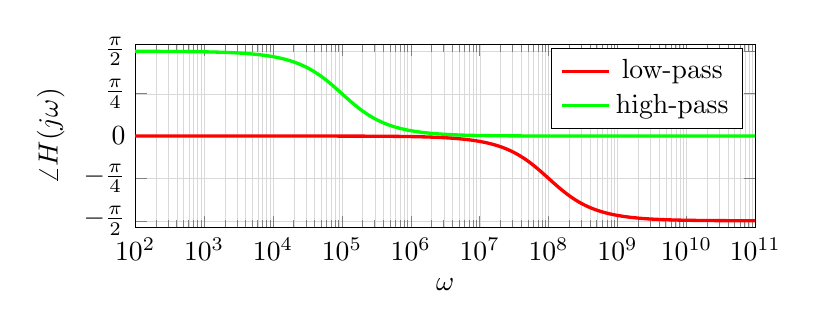
\begin{tikzpicture}[
        declare function={
        lowpass(\omega) = -rad(atan(\omega / 10^8))
          % lowpass(\omega)= (\omega < 10^7) * (0) +
          %           and(\omega >= 10^7, \omega < 10^9) * (-pi / 4 * (log10(\omega) - 7)) +
          %           (\omega >= 10^9) * (-pi / 2)
         ;
        highpass(\omega) = pi/2 - rad(atan(\omega / 10^5))
         % highpass(\omega)= (\omega < 10^4) * (pi / 2) +
         %           and(\omega >= 10^4, \omega < 10^6) * (-pi / 4 * (log10(\omega) - 4) + pi / 2) +
         %           (\omega >= 10^6) * (0)
        ;
        }
      ]

        \begin{semilogxaxis}[
          ymin= -1.7, ymax=1.7, ylabel=$\angle H(j \omega)$,
          ytick={-pi/2, -pi/4, 0, pi/4, pi/2},
          yticklabels={$-\frac{\pi}{2}$,$-\frac{\pi}{4}$,$0$,$\frac{\pi}{4}$,$\frac{\pi}{2}$},
          xmin=10^2, xmax=10^11, xlabel=$\omega$,
          domain=10^2:10^11,
          grid=both, grid style={line width=.1pt, draw=gray!30},
          width=\textwidth * 0.78,
          height=\textwidth / 3.1,
          samples=500
        ]
          \addplot [red,very thick] {lowpass(x)};
          \addlegendentry{low-pass}
          \addplot [green,very thick] {highpass(x)};
          \addlegendentry{high-pass}
        \end{semilogxaxis}
    \end{tikzpicture}
  \end{figure}

  \begin{figure}[!h]
  \centering

    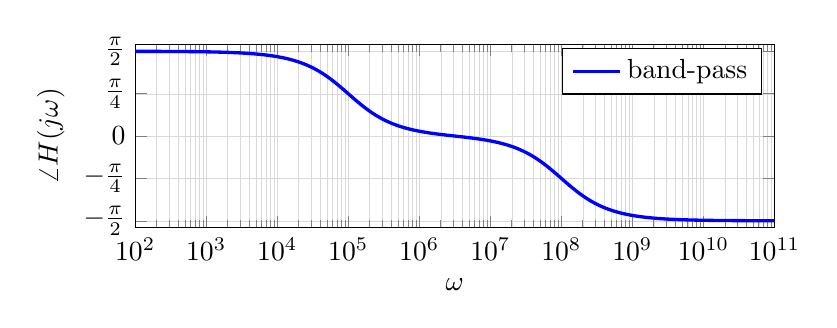
\begin{tikzpicture}[
      declare function={
      lowpass(\omega) = -rad(atan(\omega / 10^8))
        % lowpass(\omega)= (\omega < 10^7) * (0) +
        %           and(\omega >= 10^7, \omega < 10^9) * (-pi / 4 * (log10(\omega) - 7)) +
        %           (\omega >= 10^9) * (-pi / 2)
       ;
      highpass(\omega) = pi/2 - rad(atan(\omega / 10^5))
       % highpass(\omega)= (\omega < 10^4) * (pi / 2) +
       %           and(\omega >= 10^4, \omega < 10^6) * (-pi / 4 * (log10(\omega) - 4) + pi / 2) +
       %           (\omega >= 10^6) * (0)
      ;
      }
    ]

      \begin{semilogxaxis}[
        ymin= -1.7, ymax=1.7, ylabel=$\angle H(j \omega)$,
        ytick={-pi/2, -pi/4, 0, pi/4, pi/2},
        yticklabels={$-\frac{\pi}{2}$,$-\frac{\pi}{4}$,$0$,$\frac{\pi}{4}$,$\frac{\pi}{2}$},
        xmin=10^2, xmax=10^11, xlabel=$\omega$,
        domain=10^2:10^11,
        grid=both, grid style={line width=.1pt, draw=gray!30},
        width=\textwidth * 0.8,
        height=\textwidth / 3.1,
        samples=500
      ]
      \addplot [blue,very thick] {lowpass(x) + highpass(x)};
      \addlegendentry{band-pass}
      \end{semilogxaxis}
    \end{tikzpicture}
    \end{figure}

    We can add the magnitudes of the high-pass and low-pass filter graphs together because we are graphing $\log(|H(j \omega)|) = \log(|H_{high}(j \omega)| \cdot |H_{low}(j \omega)|) = \log(|H_{high}(j \omega)|) + \log(|H_{low}(j \omega)|)$.
    We can add the phases because $\angle(H_{high}(j \omega) \cdot H_{low}(j \omega)) = \angle(H_{high}(j \omega)) + \angle(H_{low}(j \omega))$.
\end{enumerate}

}

\end{enumerate}

\end{qunlist}

\end{document}
